\newpage
\section{Continued Fractions}

We're going to use some tricks involving fractions to study numbers
that have a nasty form. As an example, consider 
\[
\sqrt{2} = 1.4142135623\dots \index{sqrt2@$\sqrt{2}$}
\]
Yuck! That's just some crazy decimal. It would be nice if we could
somehow see some order in this chaos! To do this, we'll need some
definitions:

\begin{dfn}\index{continued fraction} A fraction of the form
\[
a_0 + \frac{a_1}{\displaystyle b_1 
          + \frac{a_2}{\displaystyle b_2 
          + \frac{a_3}{\displaystyle b_3 
       + \frac{a_4}{\displaystyle b_4 + \cdots
}}}}
\]
is called a \textbf{continued fraction}. If $a_1,a_2,a_3,\dots$ are
all $1$, we will call this a \textbf{simple continued fraction}.
\end{dfn}


\begin{dfn}\index{whole-number part} 
The \textbf{whole-number part} of a number is the largest whole number
which is less than or equal to the given number.
\end{dfn}

\begin{eg} 
The whole-number part of $2$ is $2$, while the whole-number part of
$5.32$ is $5$.
\end{eg}

\begin{dfn}\index{fractional part} 
The \textbf{fractional part} of a number is the number minus its
whole-number part.
\end{dfn}

\begin{eg} 
The fractional part of $2$ is $0$, while the fractional part of $5.32$
is $0.32$.
\end{eg}


\begin{ques} 
Why don't we just describe the fractional part of a number as the part
that is to the right of the decimal point? Hint: Think about
$0.99999\dots$.
\end{ques}
\QM

Given any number, we can write it as a simple continued
fraction. Consider $13/5$. To start note that
\[
3>\frac{13}{5}>2. 
\]
So this means that 
\[
\frac{13}{5}=2 + \frac{3}{5}.
\]
Here $2$ is the whole-number part and $3/5$ is the fractional part of
$13/5$. But in the simple continued fraction, our numerator is $1$,
not $3$. How do we deal with this? Well,
\[
\frac{13}{5}=2+\frac{3}{5}=2+\frac{1}{ \frac{5}{3}}.
\]
This is an improvement but we only want whole numbers in our simple
continued fractions and not $5/3$. So we write
\[
\frac{5}{3}=1+\frac{2}{3}
\]
which gives us
\[
\frac{13}{5}=2+\frac{1}{\displaystyle 1+\frac{2}{3}}.
\]
Again, we want our numerator to be $1$, not $2$ so we will repeat the steps above to get
\[
\frac{13}{5}=2+\frac{1}{\displaystyle 1+\frac{2}{3}}=2+\frac{1}{\displaystyle 1+ \frac{1}{\frac{3}{2}}} 
=2+\frac{1}{\displaystyle 1+\frac{1}{\displaystyle 1+\frac{1}{2}}}
\]
and this last expression is the simple continued fraction for $13/5$. 
We could also list our steps as:
\begin{align*}
\frac{13}{5} & = \mathbf 2 +\frac{3}{5} \\
\frac{1}{\frac{3}{5}}  = \frac{5}{3} & = \mathbf 1 + \frac{2}{3} \\
\frac{1}{\frac{2}{3}}  = \frac{3}{2} & = \mathbf 1 + \frac{1}{2} \\
\frac{1}{\frac{1}{2}} & = \mathbf 2 +0
\end{align*}
These boldface numbers tell us our continued fraction expansion.

We can also find the simple continued fraction of numbers which are
not already fractions (otherwise this would all be a bit silly).
Consider $\sqrt{2}$, remember how yucky it was?
\[
\sqrt{2} = 1.4142135623\dots \index{sqrt2@$\sqrt{2}$}
\]
To beautify this number, note that $2>\sqrt{2}>1$. So this means that
\[
\sqrt{2} = 1 + (\sqrt{2} -1).
\]
Where $1$ is the whole-number part and $(\sqrt{2} -1)$ is the
fractional part of $\sqrt{2}$. Alright, now look at
$1/(\sqrt{2}-1)$. Again we want to separate the whole-number part and
the fractional part. With a little algebra we see that
\[
\frac{1}{\sqrt{2}-1} = \frac{\sqrt{2}+1}{2-1} = \sqrt{2}+1 =
2+(\sqrt{2}+1-2) = 2 + (\sqrt{2}-1).
\]
Now don't you get bogged down in the steps. Here it is in fast forward:
\begin{align*}
\sqrt{2} &= \mathbf{1} + (\sqrt{2} -1) \\
\frac{1}{(\sqrt{2} -1)} &= \mathbf{2} + (\sqrt{2}-1) \\
\frac{1}{(\sqrt{2} -1)} &= \mathbf{2} + (\sqrt{2}-1) \\
\frac{1}{(\sqrt{2} -1)} &= \mathbf{2} + (\sqrt{2}-1), \\
&\hspace{.5em}\vdots
\end{align*}
At each step we want:
\[
\text{number} = \text{whole-number part} + \text{fractional part}
\]
Now from the bold-faced numbers above we will make our continued fraction:
\[
\sqrt{2} = \mathbf{1} + \frac{1}{\displaystyle \mathbf{2}
          + \frac{1}{\displaystyle \mathbf{2} 
          + \frac{1}{\displaystyle \mathbf{2} 
       + \frac{1}{\displaystyle \mathbf{2} + \cdots
}}}}
\]
Beautiful!
\begin{ques} Can you explain why this works?
\end{ques}
\QM

\begin{ques} 
Do you think you could find a regular fraction equal to $\sqrt{2}$?
\end{ques}
\QM


\subsubsection{Some Hidden Beauties}

Continued fractions allow us to see patterns that are otherwise
totally hidden.

Check out $e = 2.718281828459045\dots$. \index{e@$e$}It turns out that
\[
e = 2 + \frac{1}{\displaystyle 1
          + \frac{1}{\displaystyle 2 
          + \frac{1}{\displaystyle 1 
       + \frac{1}{\displaystyle 1
          + \frac{1}{\displaystyle 4 
          + \frac{1}{\displaystyle 1 
       + \frac{1}{\displaystyle 1
          + \frac{1}{\displaystyle 6 
          + \frac{1}{\displaystyle 1 + \cdots  
}}}}}}}}}
\]

Also check out $\pi = 3.14159265358\dots$.\index{pi@$\pi$} In 1999
L.J.\ Lange found this amazing continued fraction for $\pi$:
\[
\pi = 3 + \frac{1^2}{\displaystyle 6
          + \frac{3^2}{\displaystyle 6 
          + \frac{5^2}{\displaystyle 6 
       + \frac{7^2}{\displaystyle 6 
          + \frac{9^2}{\displaystyle 6 
       + \frac{11^2}{\displaystyle 6 + \cdots
}}}}}}
\]
Wow!



\newpage

\subsection*{Problems for Section \thesection}\hrule\vspace{1ex}
\begin{enumerate}
\item Explain what the \textbf{whole-number part} and what the
  \textbf{fractional part} of a number are. Give examples.
\item Find the simple continued fraction expansion of $1/2$. Explain
  your work.
\item Find the simple continued fraction expansion of $11$. Explain
  your work.
\item Find the simple continued fraction expansion of $5/3$. Explain
  your work.
\item Find the simple continued fraction expansion of $15/11$. Explain
  your work.
\item Find the simple continued fraction expansion of $22/17$. Explain
  your work.
\item Using a calculator, find the first five terms in the simple
  continued fraction expansion of $\pi$. What number do you get by
  only considering the first term? The first four?
\item Find the simple continued fraction expansion of
  $\sqrt{5}$. Explain your work.
\item Find the simple continued fraction expansion of
  $\sqrt{10}$. Explain your work.
\item Find the simple continued fraction expansion of
  $\sqrt{17}$. Explain your work.
\item Find the simple continued fraction expansion of
  $\sqrt{26}$. Explain your work.
\item Find the simple continued fraction expansion of
\[
\frac{1 + \sqrt{5}}{2}
\]
Explain your work. Note---this is a special number, it is called the
\textit{golden ratio}. More on this later.\index{golden ratio}
\item Courtney Gibbons is someone who has a rather unusual tattoo. She
  was kind enough to let an unusual person like me take a picture of
  it.  What does her tattoo represent? Explain your reasoning.
\[
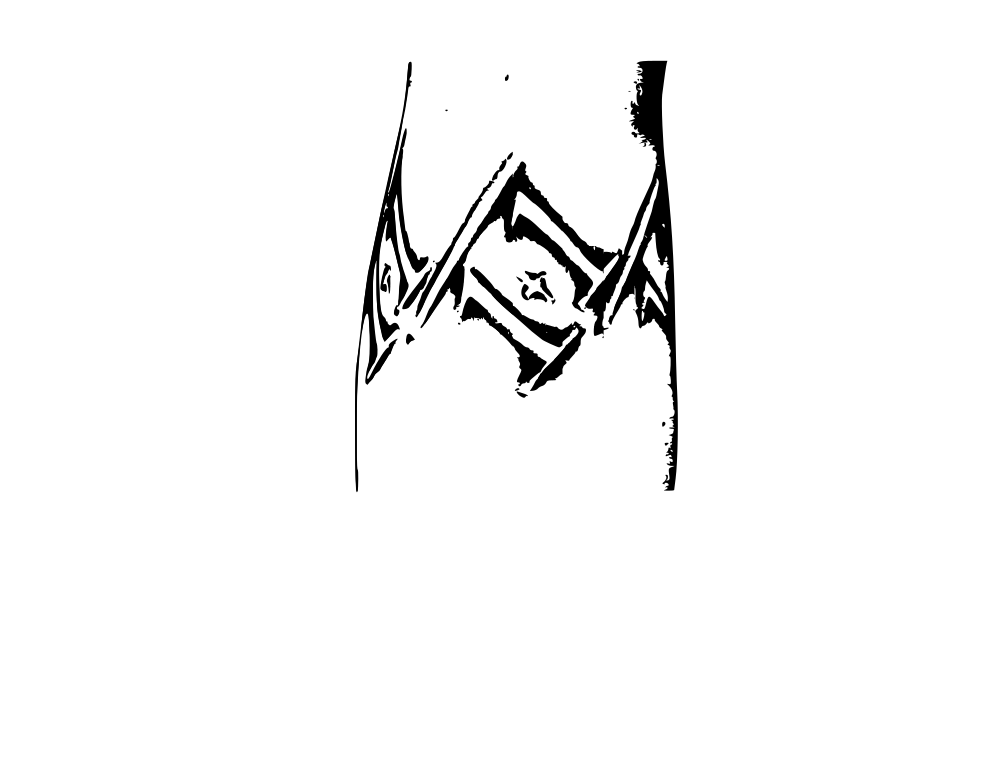
\includegraphics[width=2in]{../graphics/cgtat.pdf}
\]
\item What is it about the numbers $2,5,10,17,26$ that makes it easy
  to compute the continued fraction expansion of the square-roots of
  these numbers? Explain your answer.
\item What is the best rational approximation of $\sqrt{2}$ where the
  denominator is less than 10? Less than 20? Less than 30? Less than
  100?
\item What is the best rational approximation of $\sqrt{5}$ where the
  denominator is less than 10? Less than 20? Less than 30? Less than
  100?
\item What is the best rational approximation of $\sqrt{3}$ where the
  denominator is less than 10? Less than 20? Less than 30? Less than
  100?
\end{enumerate}

